\section{Bone transducer position}

The position of the \gls{bc} can ether be founded by subject test or literature search. Due to that the focus of the project is speech intelligibility of \gls{bc} and \gls{ac}, it have been chosen to do literature search on \gls{bc} positioning in stead of subject test. This have been chosen such that the test of speech intelligibility can be done more thorough due to more time for test planning and the more time of the test subject. The project can not offer money compensation to the test subject and therefore the time for testing position would than have lowered the time of speech intelligibility test. 

This section will compare earlier position test of \gls{bc} and conclude on a finite position.

\subsection{\gls{bc} position comparing}
The position of the \gls{bc} is important to ensure optimal condition for the subject test. Placement test for \gls{bc} have been research in several study and it have been shown that the condyle and mastoid position is the most favorable locations for optimal hearing \citep{cat_test}. The following \autoref{fig:condyle_mastoid} shows the  condyle and mastoid on a human.

\begin{figure}[H]
	\centering
		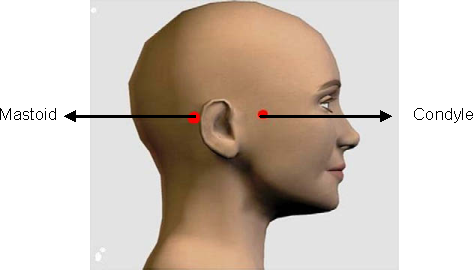
\includegraphics[width=1\textwidth]{condyle_mastoid}
		\caption{condyle and mastoid position \citep{cat_test}}
		\label{fig:condyle_mastoid}
\end{figure}

To chose the finite position of ether condyle or mastoid, the speech intelligibility and loudness perception for both position will be included in the choose. 


The article \citep{cat_test} introduce a \gls{cat} subject test, which compare  speech intelligibility with \gls{bc} position. The test is described in \autoref{ssec:cat}. \gls{fmcbct} \citep{freefield_method} compare the two position for the \gls{bc} with loudness perception. The test is done by playing a tone in a speaker where the test subject shall adjust the gain and phase of the \gls{bc} until the tone from the loudspeaker is cancelled.The following \autoref{tab:test_methoed} compare the speech intelligibility and loudness for condyle and mastoid.


Influence_without
 
\begin{table}[H]
\begin{tabularx}{\textwidth}{l X l}
\hline
\gls{cat}: & Shows that there is not statistical evidence that one of the two position of the \gls{bc} have a higher speech intelligibility over the other, but the test shows that the mean speech intelligibility score is marginal better for the mastoid. \\
\gls{fmcbct}: & Shows that there is difference in loudness perception of the two position for a B71. The test do not test the B81 because of the age of the test and therefore the result for this comparison is of the B71. The condyle is more sensitive to bone vibration that the mastoid specially in the speech intelligibility frequency range from \SI{500}{\hertz} to \SI{4000}{\hertz} where the difference is proximate \SI{5}{\decibel} \citep{freefield_method}. The exact result can be seen in the article. \\
\citep{Influence_without}: & Shows that there is difference in loudness perception of the two position for a B71. The result of the test is that there is a higher cochlear response when the \gls{bc} is at the condyle compare to the mastoid, which mean that the hearing threshold is lower at the position of condyle \citep{Influence_without} with respect to vibration of the B71. For the full result, see the article. \\ \hline
\end{tabularx}
\caption{Test result between condyle and mastoid for different intelligibility test and loudness test} 
\label{tab:test_methoed}
\end{table}



